% ---------------------------------------------------
% ----- Conclusion of the template
% ----- for Bachelor-, Master thesis and class papers
% ---------------------------------------------------
%  Created by C. Müller-Birn on 2012-08-17, CC-BY-SA 3.0.
%  Freie Universität Berlin, Institute of Computer Science, Human Centered Computing.
%
\chapter{Conclusion}
\label{chap:conclusion}

Despite neutral point of view and tralala, Wikipedia is political.
In a way, not taking a side is positioning in itself.

Special attention: following edit filters from DE Wikipedia:

196 : "US-amerikanisch -> amerikanisch ([[WP:RS\#Korrektoren]])"
and 197: "amerikanisch -> US-amerikanisch ([[WP:RS\#Korrektoren]])"
"Korrektoren sind besonders gebeten, sich an die hier vereinbarten Regeln zu halten. In Fällen, in denen verschiedene Schreibweisen zulässig sind, werden Korrektoren um taktvolle Zurückhaltung gebeten: Es ist kein guter Stil, in einer schlüssig formulierten Passage eine zulässige in eine andere zulässige Schreibweise zu ändern." from \url{https://de.wikipedia.org/wiki/Wikipedia:Rechtschreibung#Korrektoren}
Both are log only filters;
and it's a political fight

\url{http://www.aaronsw.com/weblog/wikicodeislaw}
on software is political; the software that Wikipedia runs on is political; who writes it? what values do they embed in it? (cmp also Code)

"Wikipedia’s biggest problems have come when it’s strayed from this path, when it’s given some people official titles and specified tasks. Whenever that happens, real work slows down and squabbling speeds up. But it’s an easy mistake to make, so it gets made again and again.

Of course, that’s not the only reason this mistake is made, it’s just the most polite. The more frightening problem is that people love to get power and hate to give it up. Especially with a project as big and important as Wikipedia, with the constant swarm of praise and attention, it takes tremendous strength to turn down the opportunity to be its official X, to say instead “it’s a community project, I’m just another community member”."

\cite{GeiRib2010}
"We should not fall into the trap of speaking of bots and
assisted editing tools as constraining the moral agency of
editors"

* Think about: what's the computer science take on the field? How can we design a "better"/more efficient/more user friendly system? A system that reflects particular values (vgl Code 2.0, Chapter 3, p.34)?

%************************************************************************

\section{The bigger picture: Upload filters}

Criticism: threaten free speech, freedom of press and creativity

edit filters implemented an infrastructure that enables censorship

The planned introduction of upload filters by the EU copyright reform is seen critically by Wikimedia Germany:
\begin{figure}
\centering
  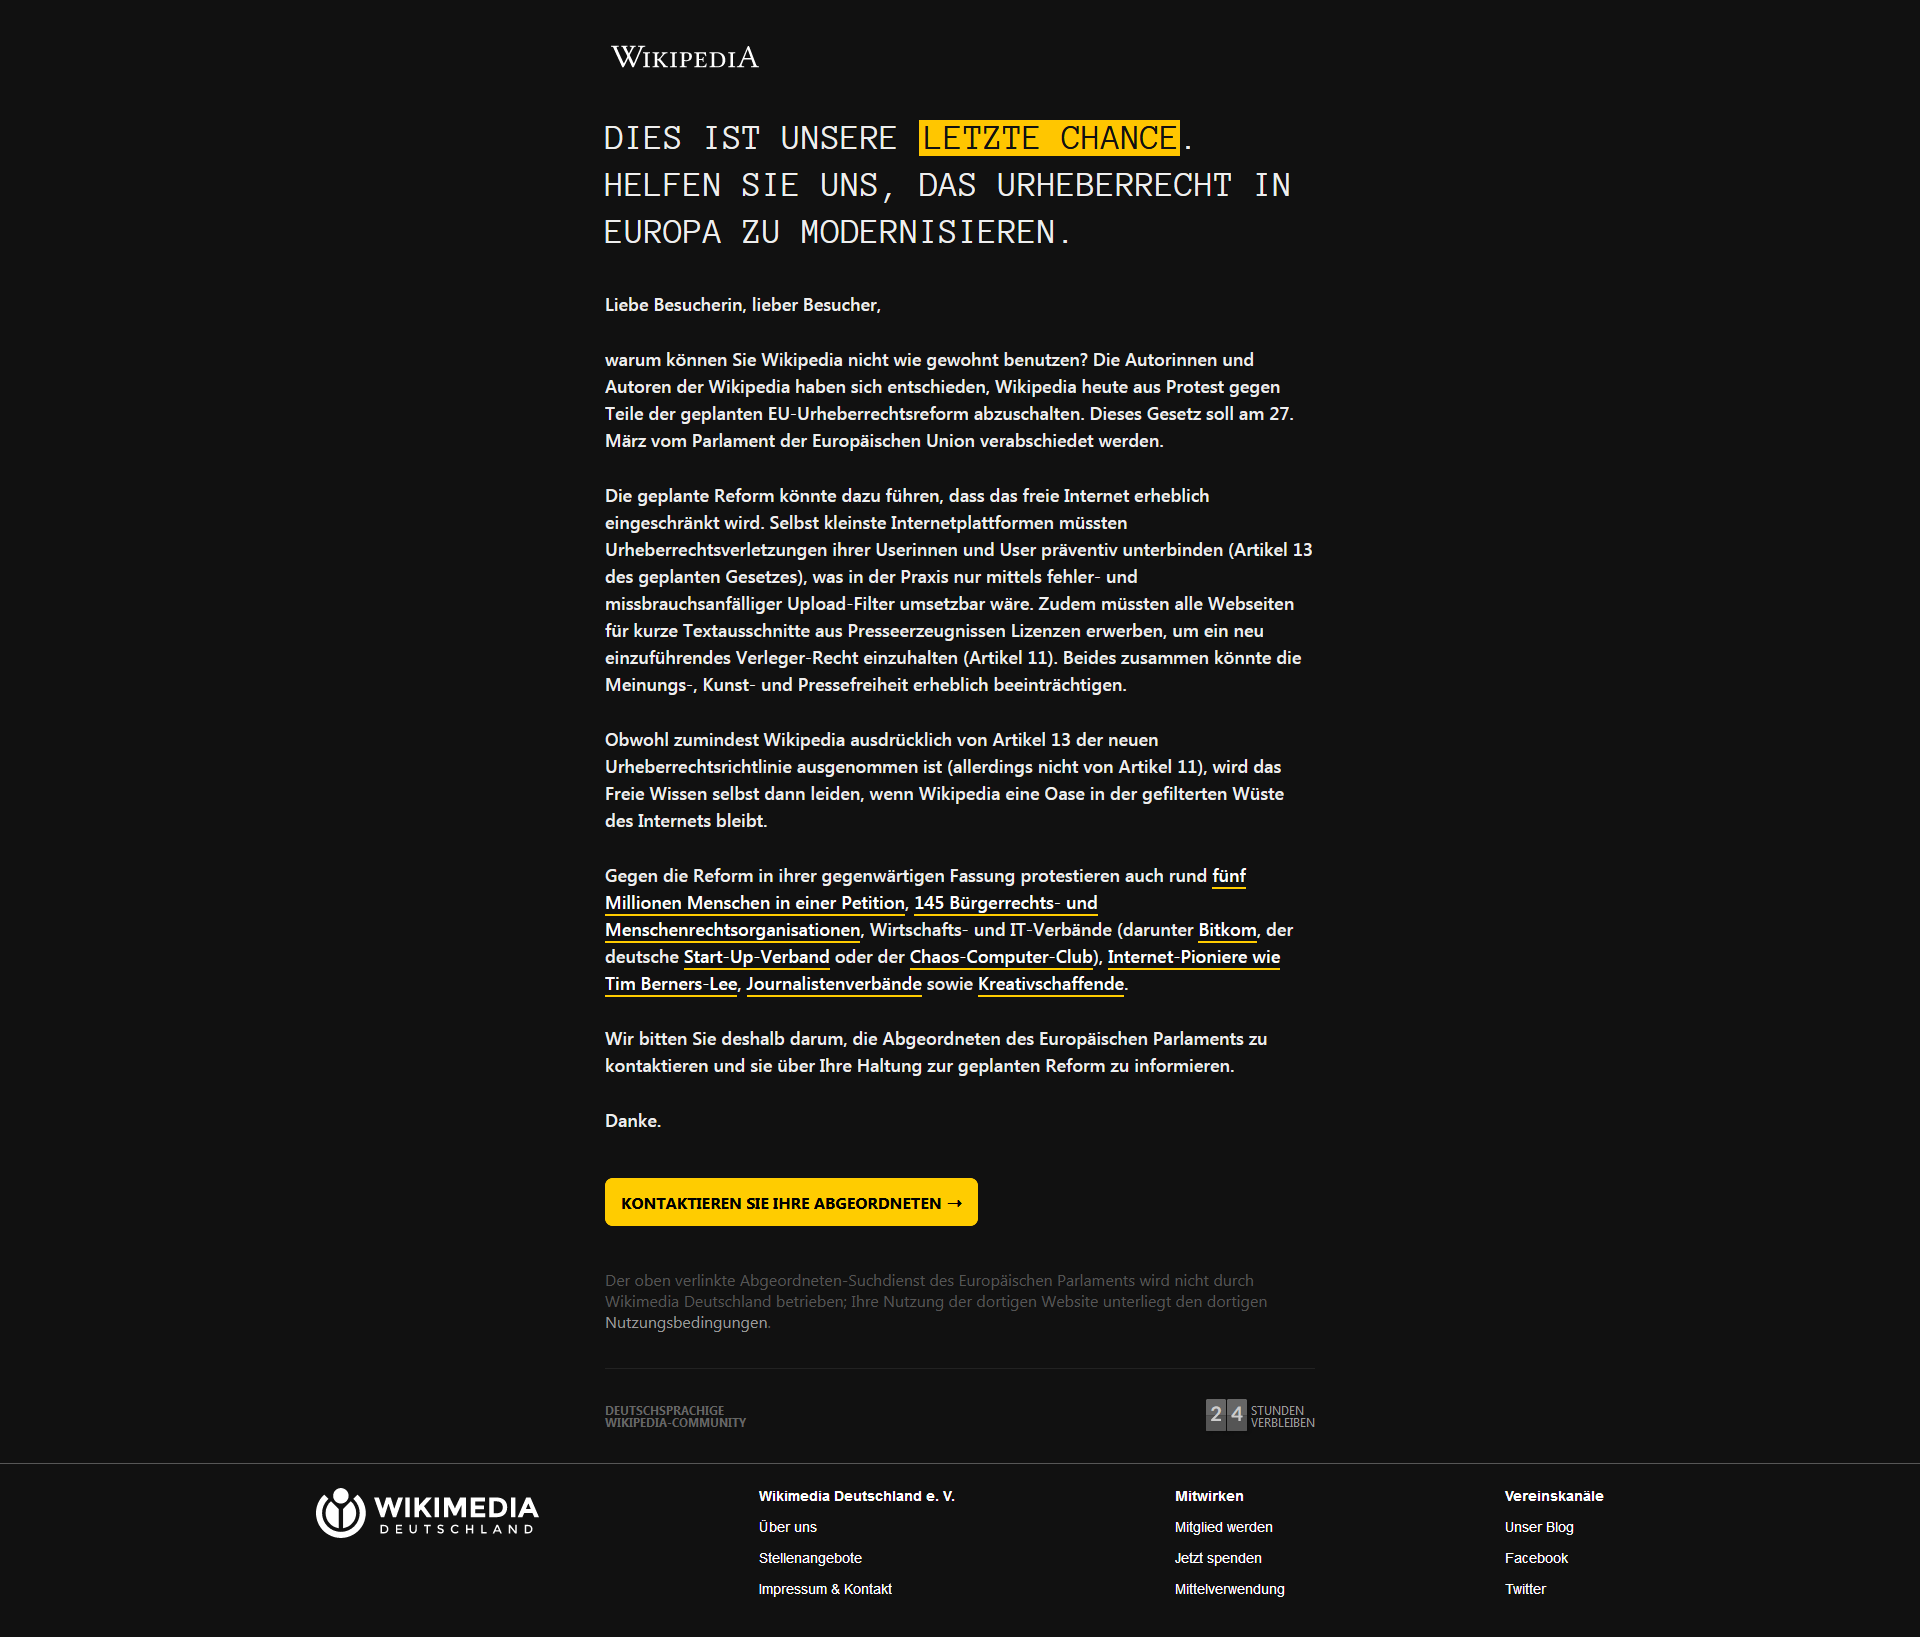
\includegraphics[width=0.9\columnwidth]{pics/Blackout_of_wikipediade_by_Wikimedia_Deutschland_-_March_2019.png}
  \caption{Blackout of wikipedia.de by Wikimedia Deutschland}~\label{fig:blackout-upload-filters}
\end{figure}

via
\url{https://de.wikipedia.org/wiki/Abschaltung_der_deutschsprachigen_Wikipedia_am_21._M%C3%A4rz_2019#/media/File:Blackout_of_wikipedia.de_by_Wikimedia_Deutschland_-_March_2019.png}

see also
\url{https://wikimediafoundation.org/2019/03/20/four-wikipedias-to-black-out-over-eu-copyright-directive/}
"Volunteer editor communities in four language Wikipedias—German, Czech, Danish, and Slovak—have decided to black out the sites on 21 March in opposition to the current version of the proposed EU Copyright Directive.

Those language editions of Wikipedia will redirect all visitors to a banner about the directive, blocking access to content on Wikipedia for 24 hours. "
"These independent language communities decided to black out in the same way most decisions are made on Wikipedia—through discussion and consensus, "

and
\url{https://wikimediafoundation.org/2019/02/28/we-do-not-support-the-eu-copyright-directive-in-its-current-form-heres-why-you-shouldnt-either/}

timeline
\url{https://edri.org/upload-filters-status-of-the-copyright-discussions-and-next-steps/}

\url{https://en.wikipedia.org/wiki/Directive_on_Copyright_in_the_Digital_Single_Market#Positions}

Interesting fact: there are edit filters that try to precisely identify the upload of media violating copyrights

%TODO refer to Lessig, Chapter 10 when making the upload filter commentary

From talk archive:
"Automatic censorship won't work on a wiki. " // so, people already perceive this as censorship; user goes on to basically provide all the reasons why upload filters are bad idea (Interlanguage problems, no recognition of irony, impossibility to discuss controversial issues); they also have a problem with being blocked by a technology vs a real person

Freedom of speech concerns
" Do we think that automatons have the judgement to apply prior restraint to speech? Do we think they should be allowed to do so even if they can be imbued with excellent judgement? We don't allow the government to apply prior restrain to speech, why would we build robots to do it? Laziness?

TheNameWithNoMan (talk) 17:39, 9 July 2008 (UTC)"

%************************************************************************

\section{Directions for further studies}
\label{sec:further-studies}
<insert long list of interesting questions here>

\begin{itemize}
	\item Die Zusammenfassung sollte das Ziel der Arbeit und die zentralen Ergebnisse beschreiben. Des Weiteren sollten auch bestehende Probleme bei der Arbeit aufgezählt werden und Vorschläge herausgearbeitet werden, die helfen, diese Probleme zukünftig zu umgehen. Mögliche Erweiterungen für die umgesetzte Anwendung sollten hier auch beschrieben werden.
\end{itemize}
